\section{Observations}\label{sec:observations}
After implementing the different techniques for the tasks posed in section~\ref{sec:tasks}, we will now describe our observations from the analysis of these different techniques. We will elaborate on the information that was retrieved from the different techniques, list their pros and cons and come up with possible improvements for the used techniques.

\subsection{Observations Task 1}
For task 1 (as described in section~\ref{sec:task1}) we implemented a Parallel Coordinate Plot (PCP) and a Scatterplot Matrix (SM). We will first argue how both techniques performed for the subtask 1a 'analyze the relations between the different attributes'. When looking at the PCP, we first try to confirm the first question we posed in section~\ref{sec:task1}: 'is there a positive relation between the attributes \texttt{AANT\_INW} and \texttt{BEV\_DICHTH}?'. When the axes of these two attributes are placed next to each other, it pretty quickly becomes apparent that this question can be answered positively. However, we also see that municipalities like Amsterdam and Rotterdam do not adhere to this. Apparently these municipalities cover such a large area that their vast number of inhabitants still not get them in the top of the \texttt{BEV\_DICHTH} scale. Municipalities like Leiden, 's-Gravenhage and Haarlem on the other hand have much less inhabitants, but score much higher on the \texttt{BEV\_DICHTH} scale because of their small surface area. If we then compare the attributes \texttt{OPP\_TOT} and \texttt{BEV\_DICHTH}, we can see there is a somewhat stronger (negative) relation between these two attributes.

In the SM it is much harder to see the positive relation between the attributes \texttt{AANT\_INW} and \texttt{BEV\_DICHTH}, and the negative relation between \texttt{OPP\_TOT} and \texttt{BEV\_DICHTH}. We can however quickly detect that there are some outliers in both of these relations. However, in the SM it is unfortunately not possible to retrieve which municipalities these outliers actually are by hovering over the dots. It was tried to implement this feature (similar to the tooltip hover in the PCP), but because the cursor already allows for brushing in the SM, it was not accomplished to also enable the tooltip feature. Being able to implement this tooltip feature could be regarded as a large improvement of the SM. On the other hand, when dots lie very close to each other, it may become hard to select a specific one.

When we return our attention to the PCP and want to compare other attributes with each other, we notice that quite some attributes have a few outliers that greatly enlarge the scale of the axis. These attributes include \texttt{OAD}, \texttt{AANTAL\_INW}, and \texttt{AANTAL\_HH}. Because of this, the majority of the lines cross the axis in a rather small area, making it very hard to distinguish between them. In its turn, this makes it harder to detect relations between attributes of the more 'general' municipalities. In order to solve this problem, a new feature is proposed. When a certain range of some attribute is selected, it may be convenient to stretch this range over the entire axis. In this way, more space is available to distribute the different lines, making it easier to distinguish between them. We should however ensure that the user is clearly notified of the fact that some data objects (municipalities) are left out in that specific view. The SM on its turn suffers from a similar usability problem. Because the plots are rather small, it is also hard to distinguish between different data objects. Here we propose to implement a zoom feature. Clicking on one of the plots would enlarge it to the size of the entire matrix, making it much more readable. However, as the implementation of both these proposed features was considered rather time-consuming, it was chosen not to do so.

Another observation that we can make when considering the PCP and SM for the task of comparing different attributes with each other, is that the SM makes it slightly easier to compare multiple attributes at once. Because all pairs of attributes are shown in one (or actually two) of the plots, we can quickly switch between comparing two attributes. When using the PCP, we need to shuffle around with the different axes and place the axes of two attributes next to each other in order to compare them.

Let us conclude the observations of subtask 1a with mentioning that performing this high-level task on the attribute set $S_{attr}$, mainly brings forward some rather obvious relations, or no clear relation at all. Examples of obvious relations are the positive one between \texttt{AANTAL\_INW} and \texttt{AANTAL\_HH}, and the negative relation between \texttt{OAD} and \texttt{STED}. A clearly unrelated pair of attributes would be \texttt{BEV\_DICHTH} and \texttt{P\_EENP\_HH}. Choosing different attributes might bring forward more interesting relations. However, with a lot of different attributes it might be hard to find those pairs that are truly valuable.



Next we continue to the second subtask: 'compare the attribute values of the different municipalities with each other'. Let us start with again shortly addressing the fact that because of the few significant outliers, the scale of some axes is stretched quite a lot, making it hard to distinguish between different data objects. This emphasizes that the solutions proposed earlier may be very valuable.

To answer to the specific question posed in section~\ref{sec:task1}, we can easily confirm from both the PCP and the SM that the four largest cities in the Netherlands score significantly highest on the \texttt{AANT\_INW} scale. Regarding the general, explorative question concerning interesting attribute distributions, we turn our attention to the \texttt{P\_EENP\_HH} attribute (i.e., municipalities with the highest percentage of single households). Looking at the top 8 ($>$ 50\%), we see that these spots are taken by the municipalities Wageningen, Groningen, Amsterdam, Delft, Utrecht, Nijmegen, Leiden, and Maastricht in descending order. Shortly considering this list, we may find it quite logical, as this list represents the top student cities in The Netherlands!

When comparing the values of a cluster of objects, there is one observation that can me made from both techniques. This observation can be made when comparing the cluster of the municipalities with a \texttt{STED} value of 1, with those with a \texttt{STED} value of 5. As becomes apparent from Figure~\ref{fig:sted}), the municipalities with a low \texttt{STED} value (i.e. the more urban municipalities), have much more fluctuating values for the other attributes. Municipalities with a \texttt{STED} value of 5 have values for the other attributes that lie much closer to each other. This again shows that there is a handful of municipalities that significantly influence the scaling.

\begin{figure}[h!]
    \centering
    \captionsetup{justification=centering,margin=0.5cm}
    \begin{subfigure}[t]{0.48\textwidth}
        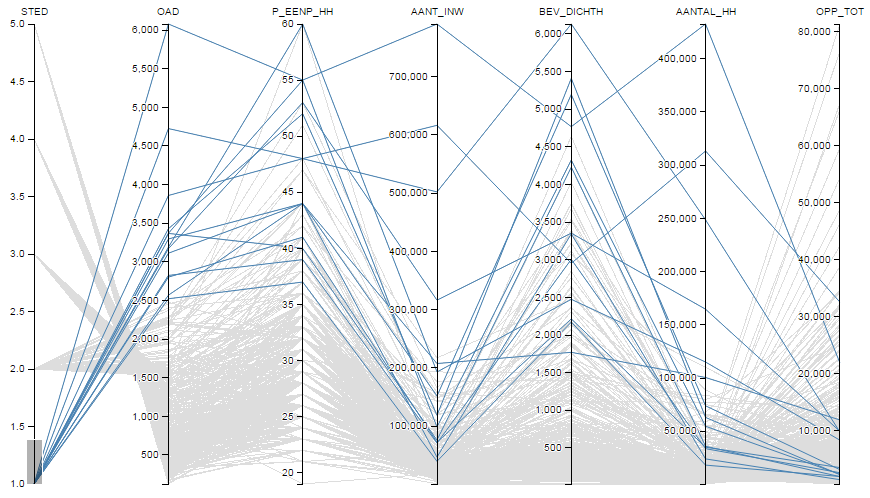
\includegraphics[width=\textwidth]{img/pcp_STED1.png}
        \caption{ }
    \end{subfigure}
    \begin{subfigure}[t]{0.48\textwidth}
        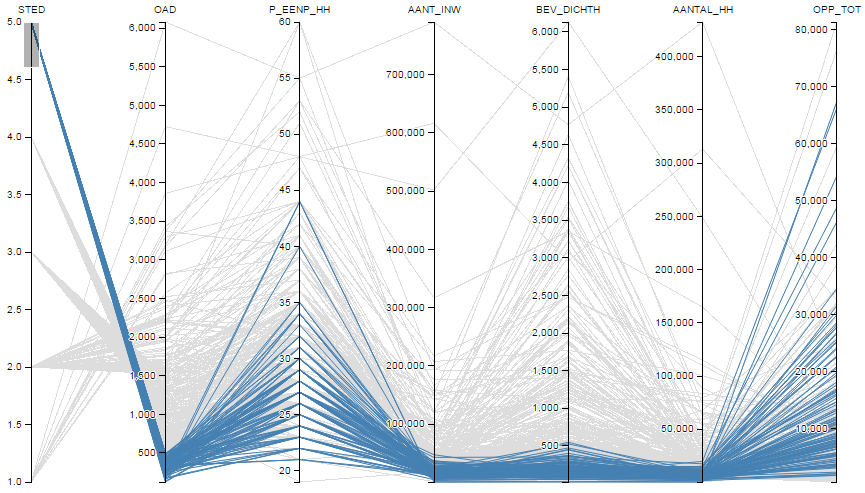
\includegraphics[width=\textwidth]{img/pcp_STED5.png}
        \caption{ }
    \end{subfigure}
    \begin{subfigure}[t]{0.48\textwidth}
        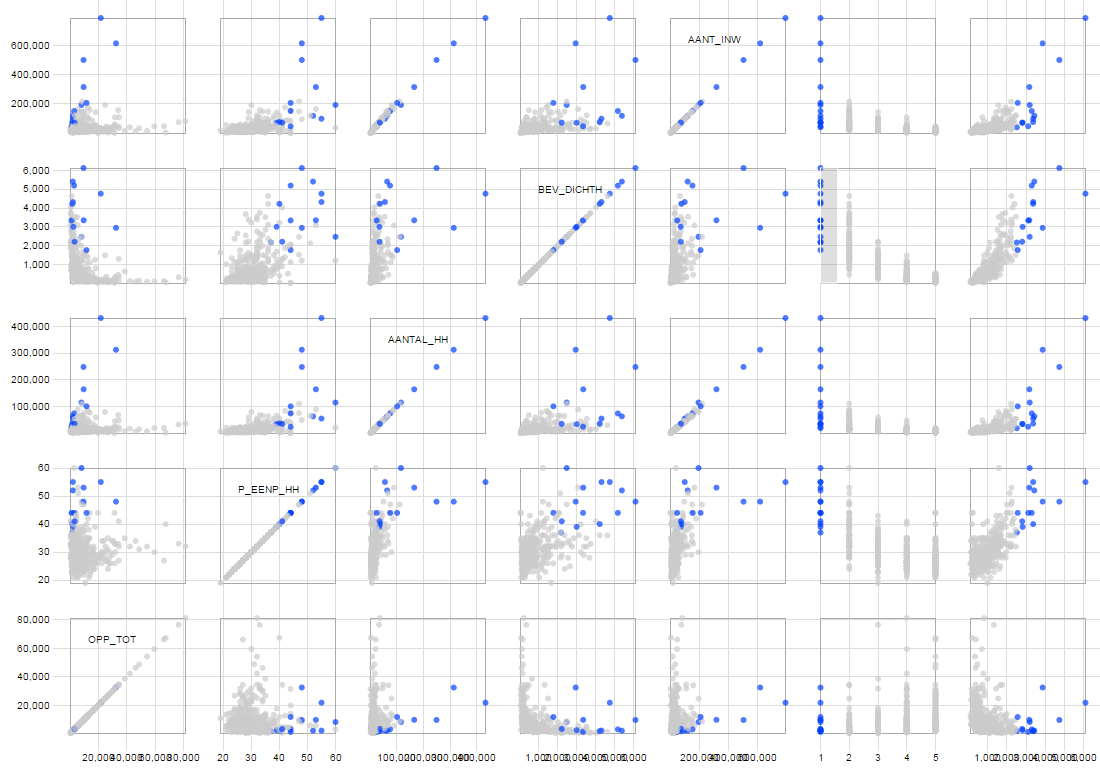
\includegraphics[width=\textwidth]{img/sm_STED1.png}
        \caption{ }
    \end{subfigure}
    \begin{subfigure}[t]{0.48\textwidth}
        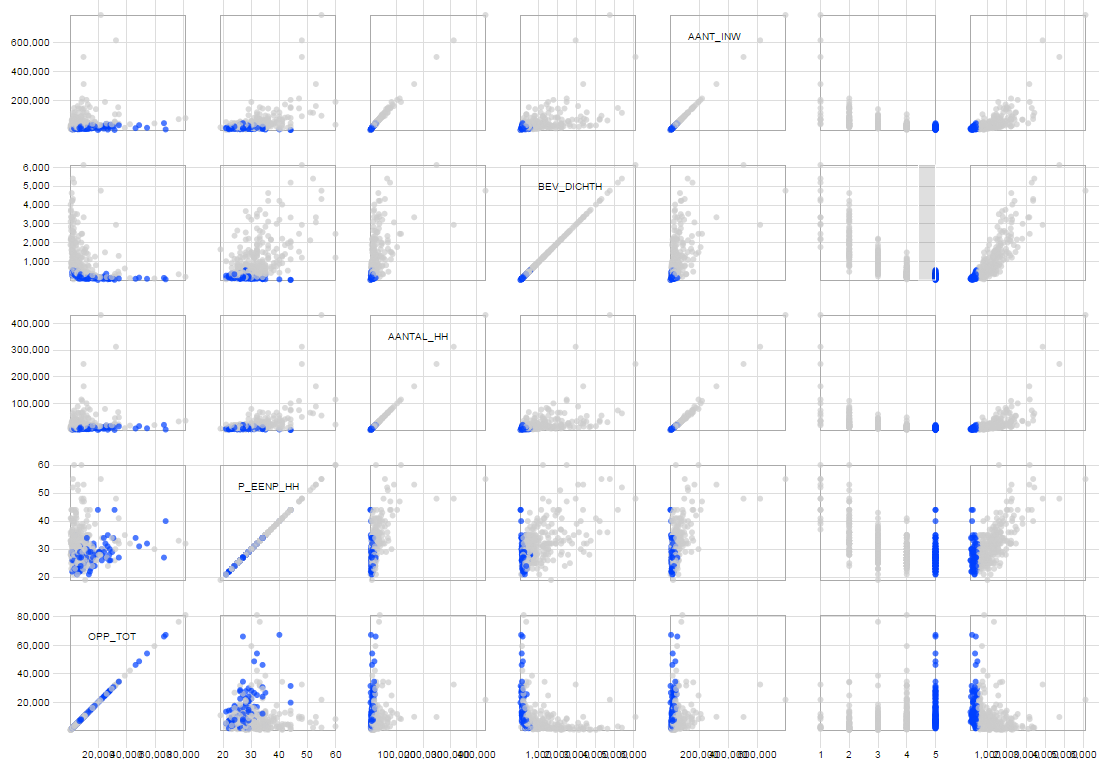
\includegraphics[width=\textwidth]{img/sm_STED5.png}
        \caption{ }
    \end{subfigure}
    \caption{Parallel Coordinate Plots highlighting the municipalities with a \texttt{STED} value of 1 (a), and a \texttt{STED} value of 5 (b), as well as the Scatterplot Matrix highlighting the municipalities with a \texttt{STED} value of 1 (c), and a \texttt{STED} value of 5 (d)}
    \label{fig:sted}
\end{figure}

Summarizing, we may conclude that both techniques are rather effective in answering the two subtasks. If we were to chose one of them, there may be  slight preference for the PCP. However, when all the proposed improvements were to be implemented, the SM might perform just as well, if not better. In general, we can conclude that this broad and high-level exploratory task may remain rather difficult with any visualization technique.


\subsection{Observations Task 2}
For this task we implemented a bar chart and choropleth map visualization. The bar chart visualization contains a combination of a regular and normalized bar chart. The choropleth map also contains an extra bar chart to give detailed information about the age groups of a certain municipality.

The specific question that these visualisations should confirm is whether there are municipalities in the Netherlands that suffer from a high degree of an aging population, and which ones do so the most. Both visualizations achieve this task in their own way. The bart chart shows that the degree of aging population in some municipalities is more than half the size of the working group, which is quite a lot. It also shows that the degree of aging population is smaller in large municipalities. An example of this is Amsterdam, which is the seventh municipality when sorting the data on the percentage of degree of aging, in ascending order (see figure~\ref{fig:bar}).

The choropleth map does not directly show that there are municipalities in the Netherlands that suffer from a high degree of an aging population. This is because the color scale of the map is determined by the highest and lowest value of the degree of aging. However, when hovering over municipalities the degree of aging is shown using a tooltip. Next to this, a bar chart shown, giving a good insight about the aging degree of the municipality. Because the bar chart has a bar for each 5-year age group, it shows a detailed distribution of the age groups, which gives extra information for analysis. The downside of these 5-year bars is that the user has to combine the bars mentally in order to 'view' the 65+ group and working group. Then again, the colormap already takes care of indicating the height of the degree of aging, and the tooltip shows the 65+ percentage of the selected municipality. Even thought the map itself may not give direct insight in the aging degree, it does provide geographic information about the aging population. The map for instance shows that the north and south of the Netherlands suffer from a higher degree of aging population than the center. Another interesting observation are the few low-degree outliers. Investigating these municipalities more closely, can again find that these are the municipalities that contain a large student city. The most notable example of this is Groningen (see figure~\ref{fig:map}).

When looking at the choropleth map, there are a few improvements and design decisions that we should shortly address. A clear improvement would for instance be adding a color scale to the map, showing the range of values that the colors in the map represent. Currently the bar chart or tooltip is required to get an idea about the value of a certain color. This color scale would even answer the question of task 2 without any need of the bar chart, because the percentage of aging population is immediately visible to the user. Furthermore we could argue that changing the hover function by a mouse click function would be an improvement. With the current hover function it is hard to compare two specific municipalities, because the moving from one municipality to another one, triggers the map to show the bar charts of all intermediate municipalities. This creates a chaotic view, and could be prevented by using a mouse click selection, rather than the hover selection. Finally we can argue about the color palette of the map. In the current choropleth map the color scale is green-red. By using these colors, the map also emphasizes municipalities with a low degree of aging population, like student municipalities. Though this is interesting information, it is not necessary to perform the specified task. Instead of the green-red color palette we could use a white-red color scale. This gives a more organized and calm impression, as shown in figure~\ref{fig:map}.

The bar chart on the other hand is more straightforward. However, a feature that would be nice to add is an absolute sort-on-population option. The bar chart is currently sorted on the percentage of 65+ population per municipality. If the bar chart could be sorted on the absolute value of 65+ inhabitants this might provide valuable additional information.

When comparing both visualizations, we may conclude that the bar chart is a better visualization technique for the task that was formulated. The user can immediately answer the question because of the sorting ption, which is not possible using the choropleth map. However, if the choropleth map were to be updated with the proposed improvements, it would also be a very suitable technique for performing task 2.

\begin{figure}[h!]
    \centering
    \captionsetup{justification=centering,margin=0.5cm}
    \begin{subfigure}[t]{0.48\textwidth}
        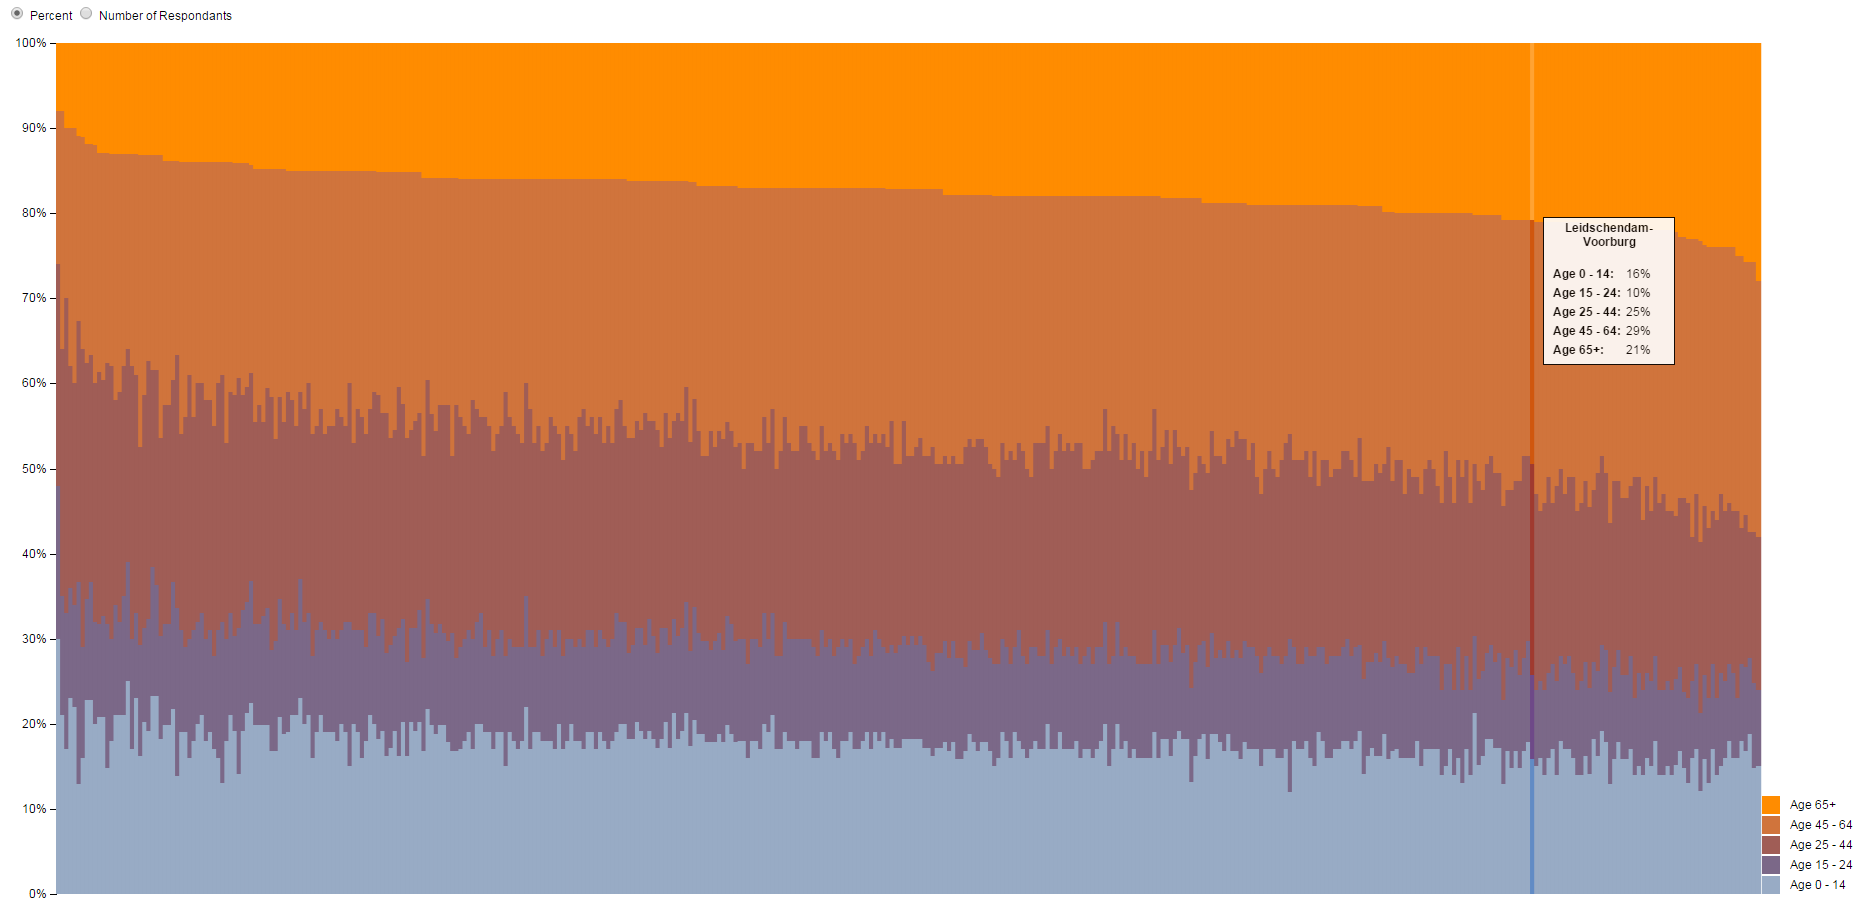
\includegraphics[width=\textwidth]{img/normalizedbarchart.png}
        \caption{ }
    \end{subfigure}
    \begin{subfigure}[t]{0.48\textwidth}
        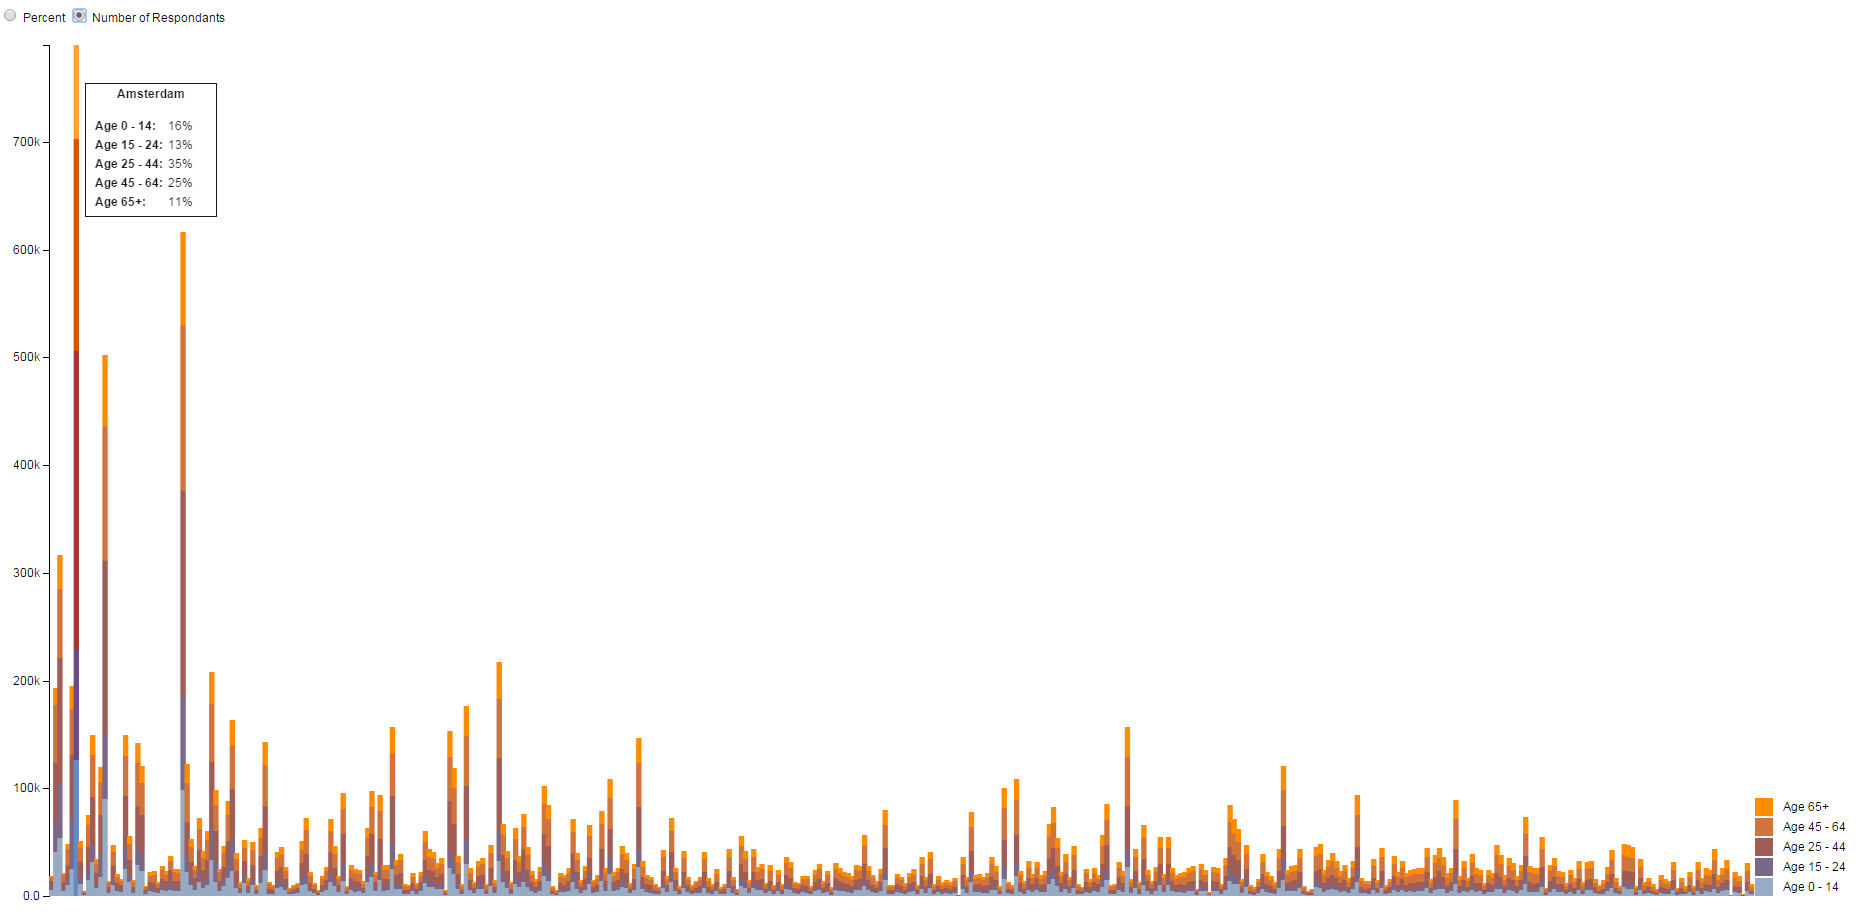
\includegraphics[width=\textwidth]{img/normalbarchart.png}
        \caption{ }
    \end{subfigure}
    \caption{Bar chart with the age group percentages of the municipalities (a), and the absolute population values (b)}
    \label{fig:bar}
\end{figure}

\begin{figure}[h!]
    \centering
    \captionsetup{justification=centering,margin=0.5cm}
    \begin{subfigure}[t]{0.48\textwidth}
        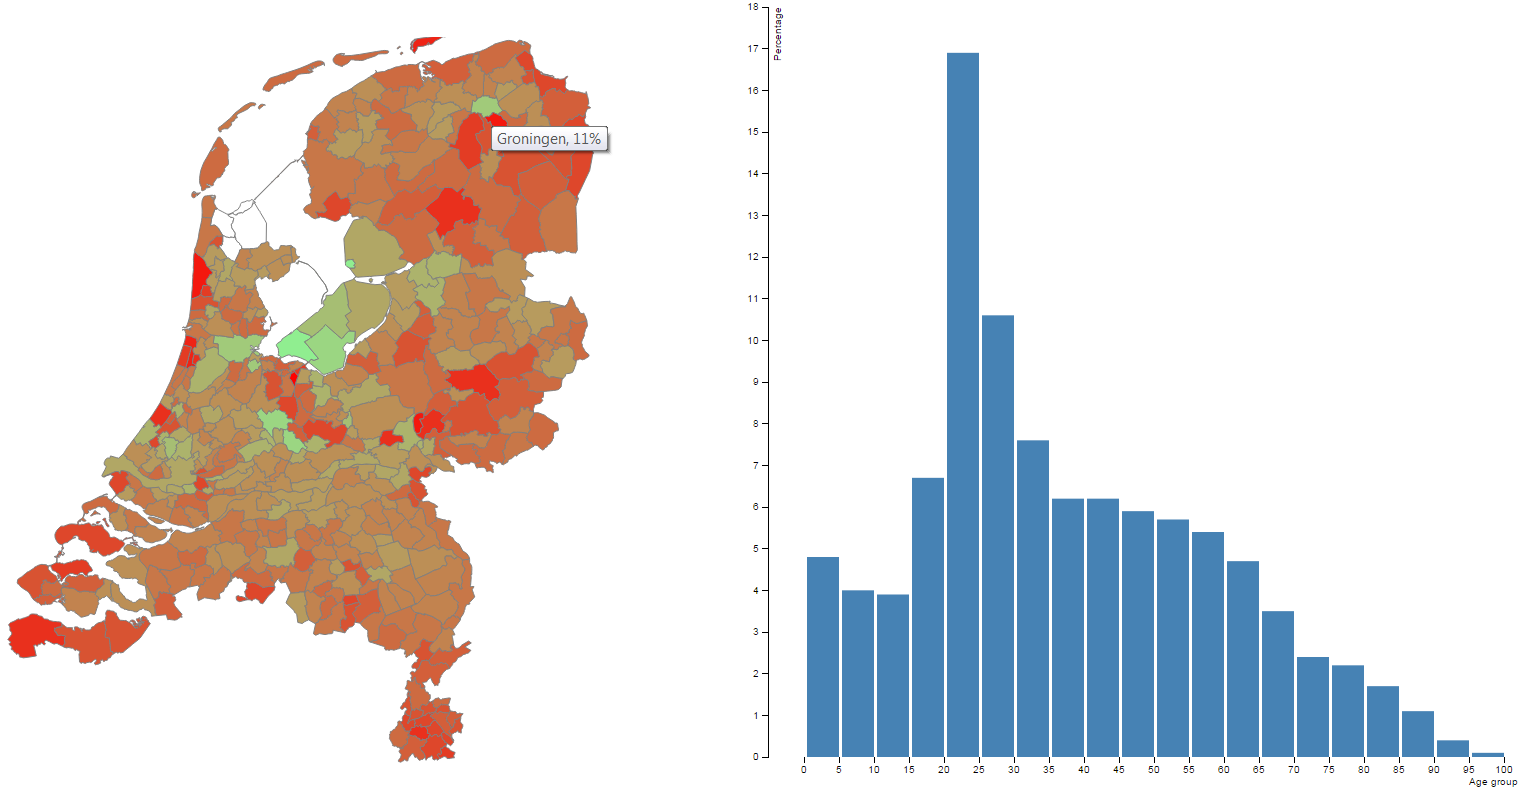
\includegraphics[width=\textwidth]{img/agemapstudent.png}
        \caption{ }
    \end{subfigure}
    \begin{subfigure}[t]{0.48\textwidth}
        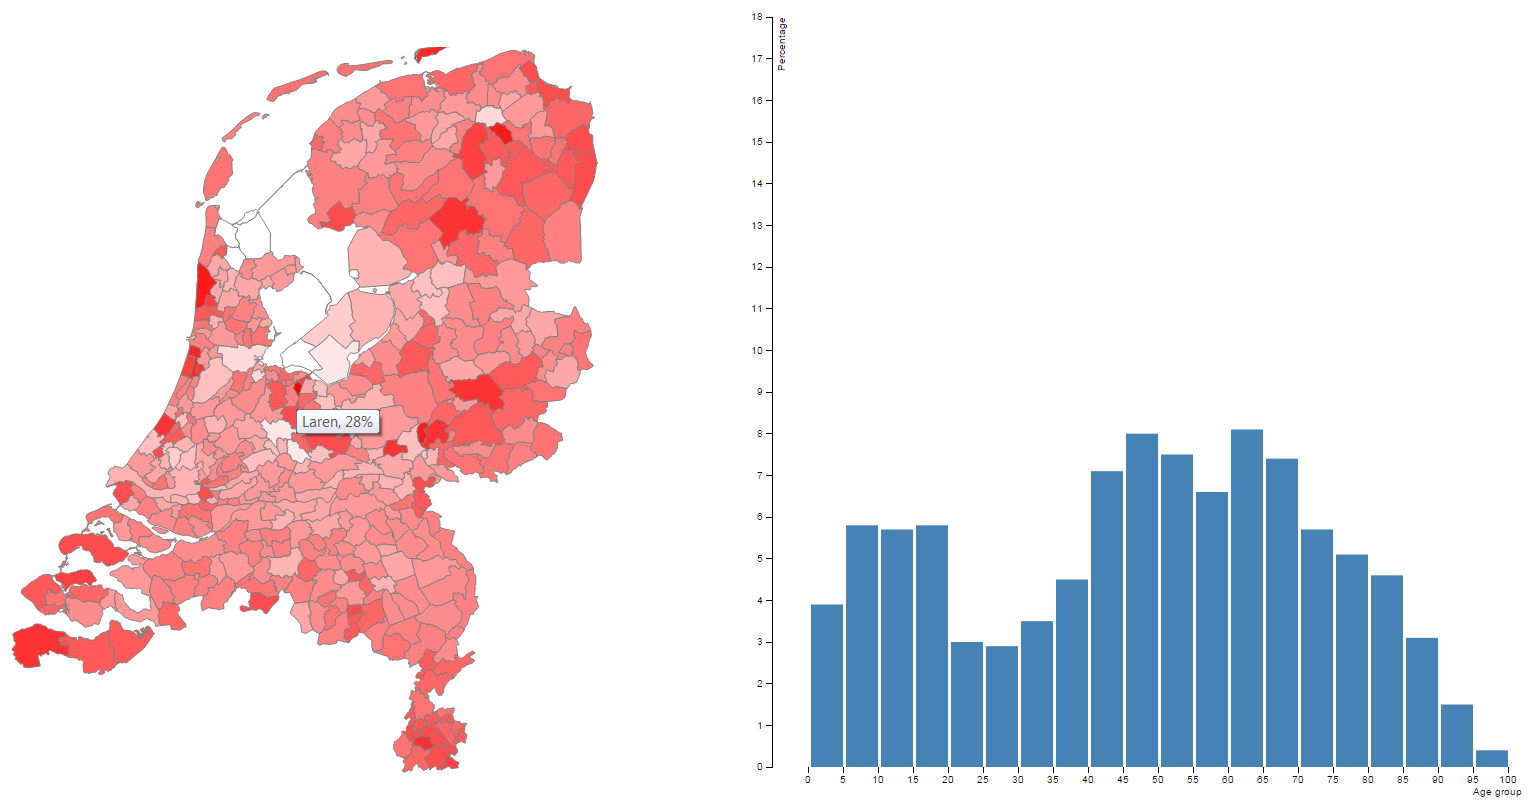
\includegraphics[width=\textwidth]{img/agemapcolor.png}
        \caption{ }
    \end{subfigure}
    \caption{Choropleth map that shows the degree of aging population using a green-red color scale (a), and the same map using a white-red color scale (b)}
    \label{fig:map}
\end{figure}
